\documentclass{projetofinal-dcc}
%%%%%%%%%%%%%%%%%%%%%%%%%%%%%%%%%%%%%%%%%%%%%%%%%%%%%%%%%%%%
%P A C O T E S
%%%%%%%%%%%%%%%%%%%%%%%%%%%%%%%%%%%%%%%%%%%%%%%%%%%%%%%%%%%%
% Adicione aqui seus pacotes
\usepackage{amssymb}
\usepackage{algorithmic}
\usepackage{algorithm}
\newcommand*{\captionsource}[2]{%
  \caption[{#1}]{%
    #1%
    \\\hspace{\linewidth}%
    \textbf{Fonte:} #2%
  }%
}
%%%%%%%%%%%%%%%%%%%%%%%%%%%%%%%%%%%%%%%%%%%%%%%%%%%%%%%%%%%%
%I N I C I O  D O  D O C U M E N T O
%%%%%%%%%%%%%%%%%%%%%%%%%%%%%%%%%%%%%%%%%%%%%%%%%%%%%%%%%%%%
\begin{document}

% título da tese é obrigatório
\title{Máquina de Vetores de Suporte Paralelo}

% autor é obrigatório; máximo de 3 autores
\author{Felipe Sepulveda de Faria}{Quero agradecer, em primeiro lugar, a Milman, pela força e coragem durante toda esta longa caminhada.

Agradeço também a todos os professores que me acompanharam durante a graduação, em especial a Profa. Silvana Roseto e ao Prof. Aloísio Pina, responsáveis pela realização deste trabalho.

Agradeço meus pais pelo apoio emocional e financeiro ao longo de toda minha graduação (Myrian e Paulo), meus irmãos (Rita, Maria Clara e Marcos), meus amigos por fazer dessa jornada mais prazerosa embora um pouco mais longa do que precisava ser.

E o que dizer a você Ana? 
Obrigada pela paciência, pelo incentivo, pela força e principalmente pelo carinho. 
Valeu a pena toda distância, todo sofrimento, todas as renúncias... Valeu a pena esperar... Hoje estamos colhendo, juntos, os frutos do nosso empenho!
Esta vitória é muito mais sua do que minha!!!}
%\author{Nome completo aluno 2}{Quero agradecer, em primeiro lugar, a Milman, pela força e coragem durante toda esta longa caminhada.

Agradeço também a todos os professores que me acompanharam durante a graduação, em especial a Profa. Silvana Roseto e ao Prof. Aloísio Pina, responsáveis pela realização deste trabalho.

Agradeço meus pais pelo apoio emocional e financeiro ao longo de toda minha graduação (Myrian e Paulo), meus irmãos (Rita, Maria Clara e Marcos), meus amigos por fazer dessa jornada mais prazerosa embora um pouco mais longa do que precisava ser.

E o que dizer a você Ana? 
Obrigada pela paciência, pelo incentivo, pela força e principalmente pelo carinho. 
Valeu a pena toda distância, todo sofrimento, todas as renúncias... Valeu a pena esperar... Hoje estamos colhendo, juntos, os frutos do nosso empenho!
Esta vitória é muito mais sua do que minha!!!}
%\author{Nome completo aluno 3}{Quero agradecer, em primeiro lugar, a Milman, pela força e coragem durante toda esta longa caminhada.

Agradeço também a todos os professores que me acompanharam durante a graduação, em especial a Profa. Silvana Roseto e ao Prof. Aloísio Pina, responsáveis pela realização deste trabalho.

Agradeço meus pais pelo apoio emocional e financeiro ao longo de toda minha graduação (Myrian e Paulo), meus irmãos (Rita, Maria Clara e Marcos), meus amigos por fazer dessa jornada mais prazerosa embora um pouco mais longa do que precisava ser.

E o que dizer a você Ana? 
Obrigada pela paciência, pelo incentivo, pela força e principalmente pelo carinho. 
Valeu a pena toda distância, todo sofrimento, todas as renúncias... Valeu a pena esperar... Hoje estamos colhendo, juntos, os frutos do nosso empenho!
Esta vitória é muito mais sua do que minha!!!}

% orientador é obrigatório
\advisor[Prof.]{Silvana Rossetto,~M.Sc.}{}

% co-orientador é opcional
\coadvisor[Prof.]{Aloísio Pina,~M.Sc.}{}

% máximo de 3 integrantes da banca (orientador e co-orientador já são adicionados automaticamente)
\banca[Prof.]{Nome do participante banca 1,~D.Sc.}{COPPE~-~UFRJ}
\banca[Prof.]{Nome do participante banca 2,~Ph.D.}{COPPE~-~UFRJ}
%\banca[Prof.]{Nome do participante banca 3,~Ph.D.}{COPPE~-~UFRJ}

\location{Rio~de~Janeiro}{RJ}{Brasil}

% mês e ano de defesa
\date{Maio}{2016}
\maketitle

\startdocument
%%%%%%%%%%%%%%%%%%%%%%%%%%%%%%%%%%%%%%%%%%%%%%%%%%%%%%%%%%%%
%A G R A D E C I M E N T O S
%%%%%%%%%%%%%%%%%%%%%%%%%%%%%%%%%%%%%%%%%%%%%%%%%%%%%%%%%%%% 
\makethankspage

%%%%%%%%%%%%%%%%%%%%%%%%%%%%%%%%%%%%%%%%%%%%%%%%%%%%%%%%%%%%
%R E S U M O
%%%%%%%%%%%%%%%%%%%%%%%%%%%%%%%%%%%%%%%%%%%%%%%%%%%%%%%%%%%%
\begin{abstract}{
  Uma Maquina de Vetores de Suporte (MVS) é um método de aprendizado de máquina supervisionado. %silvana: dizer que consiste de duas etapas: treinamento e classificação e que um conjunto de dados é usado para treinar e outro par classificar....

Seu modelo é binário de forma que após o treinamento é possível classificar um exemplo entre duas classes.

%silvana: A etapa de treinamento consiste em...
Seu treinamento consiste em iterar diversas vezes sobre todo o conjunto de treinamento realizando operações complexas no processo. 
%silvana: é possível dar uma ideia do que são essas "operações complexas"? o que caracteriza sua complexidade?

%silvana: Na etapa de classificação as mesmas operações são executadas sobre os dados de entrada...
Para classificação ela separa um subconjunto e realiza as mesmas operações sobre elas para chegar em uma estimativa. 

%silvana: Esse processo é muito custoso computacionalmente... para garantir a precisão desejada na etapa de classificação...
Esse processo é muito custoso já que as operações são complexas e um conjunto de dados precisa ser grande para render boa precisão na classificação. 
Por isso é um método interessante para ser paralelizado em GPU. GPUs possuem uma capacidade de processamento paralelo muito acima das CPUs, mas o seu uso não é trivial e é preciso adaptar os algoritmos à sua arquitetura. 

Nesse trabalho implementamos um programa capaz de rodar uma Maquina de Vetores de Suporte de forma sequencial e paralela. O algoritmo escolhido para implementar foi Kernel-Adatron, 

%silvana: por ser um algoritmo simples de MVS com potencial de ganho com a paralelização em GPU...
por ser um algoritmo que resolve os problemas da maquina de vetores de suporte pela força bruta, tem um alto potencial de ganho com paralelização em GPU. 

%silvana: avaliamos o algoritmo em relação à precisão obtida na classificação e ao ganho de desempenho da versão paralela em relação à versão sequencial.
Avaliamos o desempenho do programa tanto pelo lado da MVS quanto pela GPU, o objetivo é encontrar o maior ganho de velocidade da GPU e o maior ganho de precisão da MVS.

}
\end{abstract}

%%%%%%%%%%%%%%%%%%%%%%%%%%%%%%%%%%%%%%%%%%%%%%%%%%%%%%%%%%%%
%A B S T R A C T
%%%%%%%%%%%%%%%%%%%%%%%%%%%%%%%%%%%%%%%%%%%%%%%%%%%%%%%%%%%%
\begin{englishabstract}{
  In this project I describe the development of a binary classifier using a support vector machine algorithm known as Kernel - Adatron Algorithm for Sequential and parallel versions. The parallel version runs on GPU using it's SIMD model (Single Instruction Multiple Data ). I latter analyze the different performance in time and accuracy between the various versions and changing the algorithm's parameters.
}
\end{englishabstract}

%%%%%%%%%%%%%%%%%%%%%%%%%%%%%%%%%%%%%%%%%%%%%%%%%%%%%%%%%%%%
%L I S T A S
%%%%%%%%%%%%%%%%%%%%%%%%%%%%%%%%%%%%%%%%%%%%%%%%%%%%%%%%%%%%
% Figuras
\makefigurespage

% Tabelas
\maketablespage

% Algoritmos
\makelistingspage

% Símbolos (devem estar em ordem alfabética)
\makesymbolspage{\item [CUDA] Compute Unified Device Architecture
\item [SVM] Support Vector Machine
\item [MVS] Máquina de Vetores Suporte
\item [GPU] Graphics Processing Unit
\item [CPU] Central Processing Unit
\item [KTT] Karush-Kuhn-Tucker
\item [KAA] Kernel-Adatron Algorithm}

% Sumário 
\maketocpage

%%%%%%%%%%%%%%%%%%%%%%%%%%%%%%%%%%%%%%%%%%%%%%%%%%%%%%%%%%%%
%C O N T E Ú D O
%%%%%%%%%%%%%%%%%%%%%%%%%%%%%%%%%%%%%%%%%%%%%%%%%%%%%%%%%%%%
\startcontent
\chapter{Introdução}\label{chp:LABEL_CHP_1}

\emph{Support vector machine}, ou máquina de vetores suporte (MVS), é um método de aprendizado de máquina em que, a partir de um conjunto de dados definidos como exemplos, são definidos hiperplanos que separam as classes. Cada exemplo é composto por atributos e uma classe. Atributos são variáveis cujos valores podem ser usados para fazer a predição da classe. Um exemplo onde se desconhece a classe é chamado de caso teste. A máquina de vetores suporte representa os casos teste como pontos em um espaço $n$ dimensional, onde $n$ é o número de atributos do caso teste. A MVS cria um hiperplano que divide esse espaço de forma que seja possível identificar a qual classe o exemplo pertence.
Esse hiperplano é construído a partir da fronteira entre o subespaço ocupado por cada classe. Os pontos que definem essas fronteiras são chamados de vetores suporte.

Neste trabalho, implementamos um algoritmo de MVS que encontra esse hiperplano, avaliando todos os casos teste do conjunto de treinamento e convergindo em direção ao hiperplano que melhor divide o espaço entre os pontos de cada classe. Esse algoritmo é muito custoso computacionalmente, pois é preciso comparar todos os pares de exemplos do conjunto de treinamento a cada iteração.
Desse modo, como temos um conjunto de dados grande e um algoritmo custoso e repetitivo, temos um caso forte para a paralelização.


\par
%silvana: Existem diferentes ambientes para programação paralela, entre eles as GPUs têm ganhado destaque nos último anos...
%Para paralelização escolhi a GPU. 
Existem diferentes ambientes para programação paralela, entre os quais as GPUs (\emph{Graphics Processing Units}) têm ganhado destaque nos último anos. As GPUs tradicionalmente são usadas para computação gráfica e foram otimizadas para processar imagens e espaços com um conjunto enorme de pontos. Entretanto, essa capacidade de processar uma grande quantidade de dados em paralelo tem utilidade em muitos outros campos além dá computação gráfica, onde é necessário um alto nível de paralelismo de dados, como é o caso da MVS.
%silvana: acrescentar dizendo que tipos de problemas se adequam para implementação em GPU (forte paralelismo de dados, como é o caso de MVS...) 
%Felipe: melhor?

\par
A implementação de um MVS usando GPU não é novidade. Catanzaro, Sundaram e Keutzer em 2008 \cite{art:REF_ART_1} mostraram que uma MVS utilizando a arquitetura paralela da GPU poderia ser muito mais rápida. Eles compararam seu desempenho com o LIBSVM \cite{art:LIBSVM}, uma das bibliotecas mais populares e mais completas de MVS, o ganho foi de 9 a 35 vezes melhor no treinamento e de 81 a 138 vezes melhor na classificação. Catanzaro et al. usou o algoritmo SMO, \emph{Sequential Minimal Optimization}, que divide o problema de otimização em problemas menores.
\par
Austin Carpenter em 2009 \cite{art:REF_ART_2} criticou a versão de Catanzaro por não implementar a regressão e obter precisão um pouco abaixo do LIBSVM em um dos conjuntos de dados por usar o tipo float ao invés do tipo double. As GPUs possuem mais unidades lógicas de float do que double, o que motivou a escolha de Catanzaro por velocidade sobre precisão. O programa de Carpenter implementa regressão e usa uma mistura de float e double, recuperando a precisão perdida sem perda de velocidade.
\par
Athanasopoulos et al em 2011\cite{art:REF_ART_3} expandiram a LIBSVM de forma que todas as opções da biblioteca continuam disponíveis e com a mesma precisão, mas com uma velocidade aumentada graças a paralelizações feitas usando GPU.\par


\section{Objetivo do Trabalho}\label{sec:LABEL_CHP_1_SEC_B}
O objetivo deste trabalho é desenvolver uma implementação paralela para GPU de uma máquina de vetores suporte usando o algoritmo Kernel-Adatron descrito por Colin Campbell e Nello Cristianini \cite{art:LIVRO_KAA}. Esse algoritmo é mais simples que o SMO implementado pelos artigos referenciados anteriormente, e normalmente  recomendado como uma introdução à implementação da máquina de vetores suporte.
Além de sua simplicidade, o algoritmo Kernel-Adatron é um forte candidato à implementação paralela por adotar um método repetitivo que requer um elevado esforço de processamento. %ele teria um alto potencial para mostrar melhora em uma versão paralela.
\par
Para avaliar a implementação proposta, usaremos os mesmos conjuntos de dados usados por Catanzaro e Carpenter em seus artigos. Esses conjuntos de dados podem ser encontrados no site do LIBSVM \cite{art:LIBSVM}. 

As métricas de avaliação serão o ganho de velocidade da implementação paralela e a precisão da classificação. Para a realização dos experimentos, adotaremos a técnica convencional de validação cruzada, que consiste em particionar o conjunto de dados em conjuntos disjuntos e utilizar cada partição como conjunto de validação uma vez.

\section{Organização do Texto}\label{sec:LABEL_CHP_1_SEC_C}
O restante deste texto está organizado da seguinte forma: 
\par
No Capítulo \ref{chp:LABEL_CHP_2}, descrevemos a evolução da teoria de máquinas de vetores suporte, começando com a classificação de exemplos com dois parâmetros linearmente separáveis, até as perguntas mais complexas: por que é preciso escolher a maior margem possível? como é possível classificar conjuntos que não são linearmente separáveis? como lidar com exemplos imperfeitos e ruídos? Apresentamos algumas implementações de MVS e explicamos porque escolhemos o algoritmo Kernel-Adatron.

No Capítulo \ref{chp:LABEL_CHP_3}, descrevemos as características principais da programação paralela em GPU, a vantagem de se usar a GPU em detrimento da CPU, como ela funciona, para depois descrever como usar esses recursos usando a plataforma CUDA.

No Capítulo \ref{chp:LABEL_CHP_4}, descrevemos como implementamos o Kernel-Adatron. Começamos explicando a estrutura do programa, para em seguida descrever a versão sequencial e depois a versão paralela.

No Capítulo \ref{chp:LABEL_CHP_5}, apresentamos os conjuntos de dados utilizados, o hardware utilizado e quais as métricas usadas para análise. Em seguida apresentamos os resultados dos experimentos.

Por fim, no Capítulo \ref{chp:LABEL_CHP_6}, apresentamos as conclusões deste trabalho e que modificações podem melhorar o desempenho do programa.
\chapter{Máquina de Vetores Suporte}\label{chp:LABEL_CHP_2}

%exemplo: 
%caso teste:
%classe:
%atributo

Máquina de Vetores Suporte (MVS) é uma classe de algoritmos de aprendizado de máquina que surgiu nos anos 90 \cite{cortes1995support}. Hoje em dia são usadas em diversas áreas como reconhecimento de escrita, bioinformática e mineração de dados \cite{defilippo2004maquinas}. Essencialmente é um método de aprendizado supervisionado que pode ser usado para classificação binária, onde, a partir de um conjunto de dados de treinamento, a máquina aprende a classificar um caso teste como sendo de uma de duas classes; ou multi-classe, podendo classificar entre diversas classes. Para a multi-classificação o problema é subdividido em problemas binários menores. Também é possível usar uma MVS para regressão quando se quer estimar um valor ou probabilidade em vez de uma classe. 

Abordaremos nesse trabalho a máquina classificadora binária, já que é preciso entender bem como ela funciona antes de entender os outros métodos. Seguimos o fluxo de explicação abordado no livro \cite{art:LIVRO_SVM} que expõe a teoria por trás da máquina de vetores suporte de forma bem didática.

\section{Superfícies de Decisão Lineares}
Uma forma simples de se criar um classificador é através de uma superfície de decisão linear. Dado um conjunto de dados $(\bar{x}_i,y_i)$ $i\in[1,t]$, onde $t$ é o tamanho do conjunto e $\bar{x}_i \in \mathbb{R}^n$ são os atributos de cada exemplo, tambem chamado de caso teste, e $y_i \in \{ -1,+1 \}$ que é a classe do exemplo definida como $+1$ ou $-1$, se o conjunto for linearmente separável é possível criar uma superfície de decisão linear (reta, plano ou hiperplano) que separa esse conjunto de dados.

Uma vez encontrado o plano separador, a classificação fica fácil. Como podemos ver na Figura \ref{fig:LABEL_FIG_1}, se definirmos esse plano como $\bar{d}\cdot \bar{p} = \bar{d}\cdot \bar{c}$, onde $\bar{d}$ é o vetor ortogonal ao plano, $\bar{c}$ é o vetor de deslocamento de $\bar{d}$ e $\bar{p}$ são os pontos pertencentes a reta, podemos classificar um ponto $\bar{x}$ como pertencendo a uma classe usando uma função discriminante (Equação \ref{eq:LABEL_EQ_1}) onde a classe é definida pelo sinal do resultado.

\begin{equation}
f(\bar{\alpha})=sgn((\bar{\alpha}-\bar{c})\cdot\bar{d})
    \label{eq:LABEL_EQ_1}
\end{equation}

\begin{figure}
  \centering
  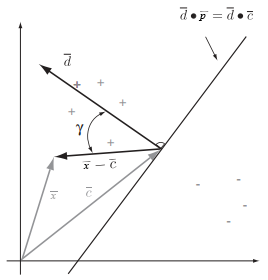
\includegraphics[width=0.4\textwidth]{imagens/svm_1.png}
  \caption{Classificação de um ponto $\bar{x}$ por uma superfície de decisão linear}
  \label{fig:LABEL_FIG_1}
\end{figure}

%silvana: definir perceptron...
%silvana: Ok!
Assumindo que nossos dados são linearmente separáveis, já sabemos qual a função discriminante, falta encontrar os parâmetros $\bar{c}$ e $\bar{d}$ que classificam corretamente esse conjunto de dados. Existem algumas formas de encontrar os parâmetros que definem essa superfície de decisão linear. Um método semelhante à máquina de vetores suporte é o perceptron \cite{art:LIVRO_SVM}. São atribuídos valores aleatórios a $\bar{c}$ e $\bar{d}$ e o perceptron classifica o conjunto de dados usando a função discriminante. A cada iteração, o perceptron corrige os valores de $\bar{c}$ e $\bar{d}$ para os dados que estiverem classificados de forma errada. Dessa forma, se o conjunto de dados for linearmente separável, o perceptron convergirá para a superfície de decisão linear.

Essa superfície separa perfeitamente os exemplos usados no treinamento, mas pode ter muitos erros para classificar outros dados. Isso ocorre porque o perceptron não tem nenhum critério para saber se a superfície é boa ou ruim. Usando a Figura \ref{fig:LABEL_FIG_2} como exemplo, suponhamos que os pontos +* e -* não estavam no conjunto de treinamento e o perceptron chegou na linha pontilhada como superfície de separação. A linha solida seria mais adequada, já que divide o espaço de forma mais justa reduzindo a chance de ter um ponto classificado errado.

\begin{figure}
  \centering
  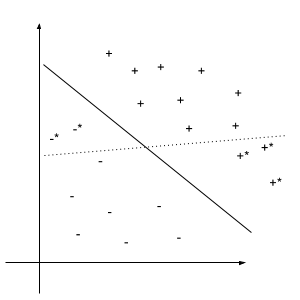
\includegraphics[width=0.4\textwidth]{imagens/svm_2.png}
  \caption{A linha sólida representa a melhor separação e a linha pontilhada representa uma separação com maior chance de erro}
  \label{fig:LABEL_FIG_2}
\end{figure}

Para encontrar essa superfície, precisamos definir hiperplanos suporte e vetores suporte. Hiperplanos suporte são as superfícies que tangenciam os dados de cada classe que queremos separar. Esses hiperplanos devem ser paralelos e a nossa superfície de decisão ótima deve se encontrar no meio desses dois hiperplanos. Vetores suporte são pontos que pertencem a esses hiperplanos de suporte.
Podemos ver na Figura \ref{fig:LABEL_FIG_3} que a superfície de decisão ótima será encontrada quando a margem entre nossos hiperplanos de suporte for máxima.

\section{Classificadores de Margem Máxima}
Classificadores de margem máxima têm como objetivo encontrar a superfície central entre duas classes de um conjunto de dados (a linha solida, na Figura \ref{fig:LABEL_FIG_2}) para minimizar a chance de erro na classificação.

\begin{figure}
  \centering
  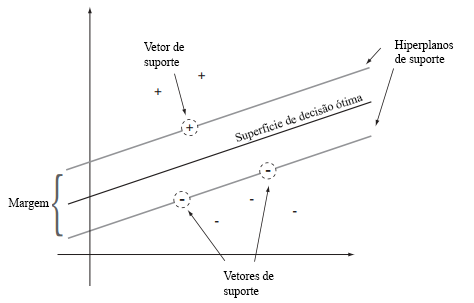
\includegraphics[width=0.7\textwidth]{imagens/svm_3.png}
  \caption{Superfície de decisão ótima e seus vetores e hiperplanos de suporte\cite{art:LIVRO_SVM}}
  \label{fig:LABEL_FIG_3}
\end{figure}

Como estamos procurando a margem máxima dado um conjunto de margens possíveis, faz sentido abordar o problema como um problema de otimização.

Formalmente, problemas de otimização são definidos como: $\underset{\bar{x}}{\min}\phi(\bar{x})$, dado que $h_i(\bar{x})\ge c_i$ $\forall \bar{x} \in \mathbb{R}^n$. Onde $\phi: \mathbb{R}^n\rightarrow \mathbb{R}$ é a função objetivo que se quer minimizar, $h_i:\mathbb{R}^n\rightarrow\mathbb{R}$ é o conjunto de funções que limitam os valores de $\phi(\bar{x})$, e $c_i$ são restrições do valor de $\bar{x}$.

Podemos então traduzir o problema de separar o conjunto de dados em um problema de otimização onde o objetivo é maximizar a distância entre os hiperplanos de suporte. Os hiperplanos suporte são hiperplanos paralelos que tangenciam os conjuntos de exemplos de cada classe e vetores suporte são pontos pertencentes a essas superfícies. Assim, o que nós queremos é a função da superfície de decisão ótima $\bar{w}^*\cdot\bar{x}=b^*$ onde a projeção entre os vetores suporte $m^*=|\bar{x}_p - \bar{x}_q|cos\gamma$, o tamanho da distancia entre os vetores multiplicado pelo coseno do ângulo entre eles, é máxima, como podemos ver na Figura \ref{fig:LABEL_FIG_4}. 

\begin{figure}
  \centering
  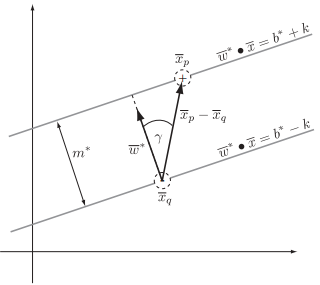
\includegraphics[width=0.6\textwidth]{imagens/svm_4.png}
  \caption{Calculando a margem $m^*$ entre os planos de suporte\cite{art:LIVRO_SVM}}
  \label{fig:LABEL_FIG_4}
\end{figure}

Para prosseguir com nossos cálculos, vamos precisar rescrever a margem ótima $m^*$ como $\frac{2k}{|\bar{w}^*|}$ (Equação \ref{eq:mEstrela}).

\begin{equation} \label{eq:mEstrela}
\begin{split}
m^* &= |\bar{x}_p-\bar{x}_q|cos\gamma\\
    &= \frac{\bar{w}^*\cdot(\bar{x}_p-\bar{x}_q)}{|\bar{w}^*|}\\
    &= \frac{\bar{w}^*\cdot\bar{x}_p-\bar{w}^*\cdot\bar{x}_q}{|\bar{w}^*|}\\
    &= \frac{(b^*+k)-(b^*-k)}{|\bar{w}^*|}\\
    &= \frac{2k}{|\bar{w}^*|}
\end{split}
\end{equation}

Queremos o vetor $\bar{w}$ que nos dê $m^*$ máximo mas para facilitar nossos cálculos mais à frente vamos reescrever nossa função objetivo como:

\begin{equation}\label{eq:funcaoObjetivo}
\begin{split}
m^*=\frac{2k}{|\bar{w}^*|} &= \max \frac{2k}{|\bar{w}|} \\
    &= \min \frac{|\bar{w}|}{2k} \\
    &= \min \frac{|\bar{w}|^2}{2k}  \\
    &= \min \frac{1}{2k} \bar{w}\cdot\bar{w}  \\
    &= \min \frac{1}{2} \bar{w}\cdot\bar{w}
\end{split}
\end{equation}

Na Função \ref{eq:funcaoObjetivo} o primeiro passo se justifica pois a maximização de uma função é igual a minimização da função inversa. O segundo passo se justifica pois o tamanho do vetor $|\bar{w}|$ é sempre positivo e a transformação de $|\bar{w}|$ para $|\bar{w}|^2$ é monotônica, então o valor de $\bar{w}$ que minimiza $|\bar{w}|$ é o mesmo que minimiza $|\bar{w}|^2$. O último passo é justificado pois a otimização não varia com a multiplicação de uma constante, assim podemos definir $k=1$ e remove-lo da equação.

Nossas restrições $h_i$ podem ser escritas como:
%Felipe: essa notação ta certa o tal que? precisa de uma chave aí?
\begin{equation}
\begin{split}
\bar{w}^*\cdot\bar{x}_i \ge b^*+k \quad \forall (\bar{x}_i,y_i)\in D \quad | \quad y_i=+1 \\
\bar{w}^*\cdot\bar{x}_i \le b^*-k \quad \forall (\bar{x}_i,y_i)\in D \quad | \quad y_i=-1 \\
\bar{w}^*\cdot\bar{x}_i \ge 1+b \quad \forall (\bar{x}_i,y_i)\in D \quad | \quad y_i=+1 \\
\bar{w}^*\cdot(-\bar{x}_i) \ge 1-b \quad \forall (\bar{x}_i,y_i)\in D \quad | \quad y_i=-1
\end{split}
\end{equation}

Essas restrições podem ser comprimidas na Equação \ref{eq:restricoesComprimidas}.

\begin{equation} \label{eq:restricoesComprimidas}
    \bar{w}^*\cdot(y_i\bar{x}_i) \ge 1+y_i b \quad \forall (\bar{x}_i,y_i)\in D
\end{equation}

Assim, um classificador por margem máxima fica definido como: dado um conjunto de dados linearmente separáveis $D=(\bar{x}_i,y_i) \subseteq \mathbb{R}^n\times\{+1,1\}$, podemos encontrar a superfície máxima de separação, $\bar{w}^*\cdot\bar{x}=b^*$, otimizando o problema $\min\phi(\bar{w},b)=\underset{\bar{w},b}{\min}\frac{1}{2}\bar{w}\cdot\bar{w}$ sujeito às restrições da Equação \ref{eq:restricoesComprimidas}.
\par

Uma máquina de vetores suporte é o problema dual do classificador de margem máxima. Podemos entender um problema dual como uma versão análoga do problema onde, ao invés de encontrar o vetor que define a superfície de separação $w$, queremos encontrar o conjunto de valores de $\bar{\alpha}$ do qual podemos inferir $w$. Para resolver esse problema dual, utilizamos a técnica dual Lagrangiana, a qual pode ser vista nos trabalhos de \cite{art:LIVRO_SVM} e \cite{art:LIVRO_KAA}.

O método de otimização Lagrangiana reescreve um problema de otimização da forma:
\begin{equation}
\underset{\bar{x}}{min}\phi(\bar{x}) \quad \text{dado que} \quad h_i(\bar{x})\ge c_i
\end{equation}
como:
\begin{equation}
\underset{\bar{\alpha}}{max} \underset{\bar{x}}{min} L(\bar{\alpha},\bar{x}) = \underset{\bar{\alpha}}{max} \underset{\bar{x}}{min}\bigg(\phi(\bar{x})-\sum_{i=1}^{l}\alpha_i g_i(\bar{x})\bigg)
    \label{eq:LABEL_EQ_7}
\end{equation}
dado que $\alpha_i\ge0$.

Para encaixarmos nosso problema no dual lagrangiano, precisamos reescrever nossas restrições como $g_i(\bar{x})=h_i(\bar{x})-c_i$. Encontrados os valores máximo de $\alpha^*$ e mínimo de $x^*$ a solução do problema dual será a mesma do problema primal, contanto que as seguintes condições se apliquem:

\begin{equation}
\begin{split}
\frac{\partial L}{\partial \bar{x}}(\bar{\alpha}^*,\bar{x})&=\bar{0}, \\
\alpha_i^*g_i(\bar{x}^*)&=\bar{0}, \\
g_i(\bar{x}^*)&\ge\bar{0} , \\
\bar{\alpha}_i^*(\bar{x}^*)&\ge\bar{0} 
\end{split}
\end{equation}

Essas condições são conhecidas como as condições de Karush-Kuhn-Tucker ou KKT, e podemos usá-las para reescrever nosso problema dependendo somente de $\bar{\alpha}$, facilitando nossa busca. Agora podemos aplicar essa técnica ao nosso problema de margem máxima, escrevendo nossa função lagrangiana como:

\begin{equation}
\begin{split}
L(\bar{\alpha},\bar{w},b) &=\phi(\bar{w},b) -  \sum_{i=1}^{l}\alpha_i g_i (\bar{w},b) \\
 &=\frac{1}{2}\bar{w}\cdot\bar{w} - \sum_{i=1}^{l}\alpha_i (y_i(\bar{w}\cdot \bar{x}_i -b)-1) \\
 &=\frac{1}{2}\bar{w}\cdot\bar{w} - \sum_{i=1}^{l}\alpha_i y_i \bar{w}\cdot \bar{x}_i + b \sum_{i=1}^{l}\alpha_i y_i + \sum_{i=1}^{l}\alpha_i\\
\end{split}
\end{equation}

Aplicando as KKTs chegamos ao nosso classificador de margem máxima dual:
\begin{equation}
    \underset{\bar{\alpha}}{max} \phi' (\bar{\alpha}) = \underset{\bar{\alpha}}{max} \Bigg( \sum_{i=1}^{l}\alpha_i - \frac{1}{2}\sum_{i=1}^{l}\sum_{j=1}^{l}\alpha_i \alpha_j y_i y_j \bar{x}_i\cdot \bar{x}_j \Bigg)
    \label{eq:EQ_Treinador_1}
\end{equation}
dado que:
\begin{equation}
    \sum_{i=1}^{l}\alpha_i y_i = 0 \quad \text{e} \quad \alpha_i \ge 0 \quad \forall  i \in \{1,l\}
    \label{eq:restricoes}
\end{equation}

Uma vez encontrado nosso $\bar{\alpha}^*$ ótimo, podemos classificar um novo ponto $\bar{x}$ com a fórmula:

\begin{equation}
    f(\bar{x}) = sgn\Bigg(
        \sum_{i=1}^{l} \alpha_i^*y_i\bar{x}_i\cdot\bar{x}
        -b^*
    \Bigg)
    \label{eq:EQ_Classificador_1}
\end{equation}

\begin{equation}
    b^* = \sum_{i=1}^{l} 
    \Bigg(
        \alpha_i^*y_i\bar{x}_i\cdot\bar{x}_{sv+} -1
    \Bigg)
    \label{eq:EQ_B_1}
\end{equation}

Onde $b^*$ representa a distância do plano à origem, $\alpha_i^*=0$ implica que $\bar{x}_i$ não influencia no resultado, $\alpha_j^*> 0$ implica que $\bar{x}_j$ é um vetor de suporte e $\bar{x}_{sv+}$ é um vetor de suporte positivo qualquer.


\section{O Truque do Kernel}
Com o que foi apresentado nas seções anteriores, conseguimos uma máquina de vetores suporte linear. Porém poucos conjuntos de dados são, na prática, linearmente separáveis. Para usar nossa máquina em conjuntos de dados que não sejam linearmente separáveis precisamos projetá-los de forma que fiquem linearmente separáveis, como na Figura \ref{fig:LABEL_FIG_5}.

\begin{figure}
  \centering
  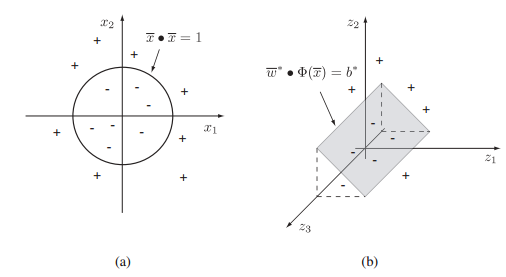
\includegraphics[width=1\textwidth]{imagens/svm_5.png}
  \caption{Em (a) não é possível separar os conjuntos de forma linear, mas transformando os dados em $\mathbb{R}^2\rightarrow \mathbb{R}^3$ em (b) conseguimos separá-los linearmente \cite{art:LIVRO_SVM}}
  \label{fig:LABEL_FIG_5}
\end{figure}

Para isso, precisamos escolher funções de projeção, $\phi:\mathbb{R}^n\rightarrow\mathbb{R}^m$, assim passamos todos nossos exemplos para um espaço de dimensão maior, na esperança que nesse espaço eles possam ser linearmente separáveis.

Podemos ver nas equações de treinamento \ref{eq:EQ_Treinador_1} e classificação \ref{eq:EQ_Classificador_1}, que sempre é avaliado o produto de dois casos teste $\bar{x}_i\cdot\bar{x}_j$, então podemos substituir $\phi(\bar{x}_i) \cdot \phi ( \bar{x}_j )$ por $k(\bar{x}_i,\bar{x}_j)$ de forma que   seja mais simples que o produto de $\phi(\bar{x})$.

Na Figura \ref{fig:LABEL_FIG_5} usamos a projeção $\phi(\bar{x})=(x_1^2,x_2^2,\sqrt{2}x_1x_2)$ e podemos simplificar seu produto (Equação \ref{eq:phiSimplificado}).

\begin{equation} \label{eq:phiSimplificado}
\begin{split}
\phi(\bar{x})\cdot \phi(\bar{y}) &= (x_1^2,x_2^2,\sqrt{2}x_1x_2) \cdot (y_1^2,y_2^2,\sqrt{2}y_1y_2) \\
&=x_1^2y_1^2+x_2^2y_2^2+2x_1x_2y_1y_2 \\
&=(x_1y_1+x_2y_2)(x_1y_1+x_2y_2) \\
&=(\bar{x}\cdot\bar{y})(\bar{x}\cdot\bar{y}) \\
&=(\bar{x}\cdot\bar{y})^2
\end{split}
\end{equation}

Chamamos essa simplificação de truque do kernel. Existe uma série de restrições que uma função tem que cumprir para ser considerada um kernel válido. Não vamos abordar aqui métodos de criação de kernels, pois é um tópico extenso, que pode ser visto em \cite{art:LIVRO_SVM}. Muitos kernels possuem uma variável livre que deve ser adaptada ao conjunto de dados estudado, podendo influenciar na sua precisão. Alguns kernels populares e suas variáveis livres podem ser vistos na Tabela \ref{tab:Kernels}.
\begin{table}
    \centering
    \caption{Kernels Populares e Suas Variáveis Livres}
    \label{tab:Kernels}
    \begin{tabular}{|c|c|c|} \hline
            Kernel & Função & Variáveis Livres \\ \hline
        Kernel Linear & $k(\bar{x},\bar{y})=\bar{x}\cdot\bar{y}$ & nenhum \\
        Kernel Homogêneo Polinomial & $k(\bar{x},\bar{y})=(\bar{x}\cdot\bar{y})^d$ & $d\ge2$ \\
        Kernel Não-Homogêneo Polinomial & $k(\bar{x},\bar{y})=(\bar{x}\cdot\bar{y}+c)^d$ & $d\ge2, c > 0$ \\
        Kernel Gaussiano & $k(\bar{x},\bar{y})=e^{-\big(\frac{|\bar{x}-\bar{y}|^2}{2\sigma^2}\big)}$ & $\sigma>0$ \\ \hline
    \end{tabular}
\end{table}

Para transformar nossa máquina de vetores suporte linear em uma máquina não linear apenas substituímos $\phi(\bar{x}_i) \cdot \phi ( \bar{x}_j )$ por $k(\bar{x}_i,\bar{x}_j)$ nas equações \ref{eq:EQ_Treinador_1}, \ref{eq:EQ_Classificador_1} e \ref{eq:EQ_B_1}.

Treinador:
\begin{equation}
    \bar{\alpha}^* = \underset{\bar{\alpha}}{argmax}{\phi}'(\bar{\alpha}) =\underset{\bar{\alpha}}{argmax} \Bigg( \sum_{i=1}^{l}\alpha_i - \frac{1}{2}\sum_{i=1}^{l}\sum_{j=1}^{l}\alpha_i \alpha_j y_i y_j k(\bar{x}_i,\bar{x}_j) \Bigg)
    \label{eq:EQ_Treinador_2}
\end{equation}

Classificador:
\begin{equation}
    f(\bar{x}) = sgn\Bigg(
        \sum_{i=1}^{l} \alpha_i^*y_i k(\bar{x}_i,\bar{x})
        -b^*
    \Bigg)
    \label{eq:EQ_Classificador_2}
\end{equation}
\begin{equation}
    b^* = \sum_{i=1}^{l}
    \Bigg(
        \alpha_i^*y_i k(\bar{x}_i,\bar{x}_{sv+})-1
    \Bigg)
    \label{eq:EQ_B_2}
\end{equation}

\section{Margem Flexível}
Conjuntos reais de dados possuem ruídos e pontos anormais que podem piorar muito a porcentagem de acertos de uma máquina de vetores suporte (Figura \ref{fig:LABEL_FIG_6}). As máquinas vistas até agora possuem margem rígida, mas também existem máquinas de vetores suporte com margem flexível que ignoram certos pontos com ruído.

Passamos a permitir que alguns pontos sejam classificados incorretamente. Definimos $\epsilon_i$ como a distância entre cada $x_i$ classificado errado e seu hiperplano de suporte, ou $0$ se o ponto estiver classificado corretamente, como pode ser visto no lado direito da Figura \ref{fig:LABEL_FIG_6}.

\begin{figure}
  \centering
  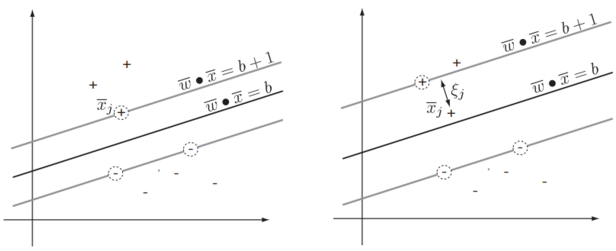
\includegraphics[width=1\textwidth]{imagens/svm_6.png}
  \caption{No exemplo da direita, ignoramos $\bar{x}_j$, que pode ser considerado ruído \cite{art:LIVRO_SVM}}
  \label{fig:LABEL_FIG_6}
\end{figure}

Para aceitar esses erros no nosso algoritmo, escolhemos uma constante $C$ que atribuímos como um peso para os erros. No problema primal, incluímos $C$ na nossa função objetivo \ref{eq:funcaoObjetivo}:

\begin{equation}
    \underset{\bar{w}, \bar{\epsilon}, b}{min}\phi(\bar{w}, \bar{\epsilon},b)
    = \underset{\bar{w}, \bar{\epsilon}, b}{min}\frac{1}{2}\bar{w}\cdot\bar{w} + C\sum_{i=1}^l \epsilon_i
    = \frac{1}{2}\bar{w}^*\cdot\bar{w}^* + C\sum_{i=1}^l \epsilon_i^*
    =m^*
\end{equation}

Queremos minimizar a função objetivo, portanto, se o peso dos erros for alto, permitimos menos erros na nossa função. No caso contrário se o peso dos erros for pequeno eles não vão influenciar tanto na função de minimização.

Concluindo,  quanto maior $C$, maior o peso dos erros e mais próximo a margem flexível fica da margem rígida. Um $C$ menor permite mais erros, fazendo com que a margem cresça e se distancie da margem rígida. No problema dual esse limite aparece como: $0\le \alpha_i \le C$

\section{Implementação}
Definimos uma máquina de vetores suporte bem robusta, capaz de classificar conjuntos de dados não lineares e suscetíveis a ruídos. A complexidade de implementação de uma MVS consiste na dificuldade de se achar os valores máximos de $\bar{\alpha}$. Existem alguns algoritmos diferentes para se chegar nesse resultado, alguns deles descritos em \cite{art:LIVRO_SVM} são apresentados a seguir.

%Felipe No livro está Gradient Ascent, não sei se essa tradução está boa
\subsection{Gradiente Ascendente}\label{sec:gradiente}
O algoritmo Gradiente Ascendente (\ref{alg:gradiente}) usa o gradiente de $\alpha$ para chegar no seu valor ótimo. O gradiente de um vetor é um vetor que aponta para a direção onde a função cresce naquele ponto. Dessa forma, podemos calcular o gradiente de $\bar{\alpha}$ em um ponto aleatório e incrementar os valores de $\bar{\alpha}$ pelo gradiente. Sabemos que chegamos no máximo local quando o gradiente for $0$, ou quando a diferença de $\bar{\alpha}$ entre as iterações é aproximadamente $0$. Nesse ponto temos o valor ótimo de $\bar{\alpha}$. Apesar de não considerarmos $b$ nessa implementação, seu valor pode ser encontrado a partir de $\bar{\alpha}$. Calculando o gradiente do nosso treinador encontrado em \ref{eq:EQ_Treinador_2} chegamos à equação \ref{eq:Gradiente}.

\begin{equation}
    \triangledown_i {\phi}'(\bar{\alpha}) = 1-y_i\sum_{j=1}^ly_j\alpha_jk(\bar{x}_j,\bar{x}_i)
    \label{eq:Gradiente}
\end{equation}

Não temos garantia de que o tamanho do gradiente não seja maior que a distância até o ponto ótimo, por isso devemos incluir uma taxa de aprendizado $\eta$ multiplicada pelo gradiente. Valores comuns de $\eta$ variam na faixa de $[0,1]$. Como o máximo da dual lagrangiana é único, podemos garantir que o algoritmo vai convergir dado um $\eta$ pequeno o suficiente.

\begin{algorithm}[h!]
\caption{Algoritmo Gradiente Ascendente}
\label{alg:gradiente}
\begin{algorithmic}[1]
\STATE $\eta>0$
\STATE $\bar{\alpha} \leftarrow \bar{0}$
\REPEAT
\STATE $\bar{\alpha_{old}} \leftarrow \bar{\alpha}$
\FOR{$i=1$ to $l$}
\STATE $\alpha_i \leftarrow a_i + \eta \triangledown_i {\phi}'(\bar{\alpha})$
\ENDFOR
\UNTIL{$\bar{\alpha}-\bar{\alpha_{old}}\approx \bar{0}$}
\RETURN $\bar{\alpha}$
\end{algorithmic}
\end{algorithm}

\subsection{Algoritmo Kernel-Adatron} \label{sec:kaa}
O problema do Gradiente Ascendente é que ele ignora as restrições de otimização \ref{eq:restricoes}, não considera o valor de $b$ e não considera uma margem flexível. O algoritmo Kernel-Adatron (\ref{alg:KAA}) resolve esses problemas. Em \cite{art:LIVRO_KAA} é explicado que a primeira restrição, $\sum_{i=1}^{l}\alpha_i y_i = 0$, só é necessária para restringir o valor de $b$ no ponto máximo. Ao fixar o valor de $b$ em zero, podemos abrir mão dessa restrição. O valor de $b$ é usado para encontrar o deslocamento da origem da nossa superfície de decisão, de forma que, fixando esse valor em zero, nos limitamos a hiperplanos que cruzem a origem no espaço de projeção. De acordo com Campbell, na prática essa generalização não prejudica os resultados quando estamos tratando de um espaço de muitas dimensões. Assim, ficamos com as restrições $\alpha_i \ge 0$ e $\alpha_i \le C$ que podem ser facilmente implementadas.

\begin{algorithm}[h!]
\caption{Algoritmo Kernel-Adatron}
\label{alg:KAA}
\begin{algorithmic}[2]
\STATE $D = \{(\bar{x_i},y_1)...(\bar{x_i},y_1)\} \subset \mathbb{R}^{n}\times \{+1,-1\}$
\STATE $\eta>0$
\STATE $C>0$
\STATE $b=0$
\STATE $\bar{\alpha} \leftarrow \bar{0}$
\REPEAT
\STATE $\bar{\alpha_{old}} \leftarrow \bar{\alpha}$
\FOR{$i=1$ to $l$}
\STATE $\alpha_i \leftarrow min\big\{C,max\big\{0,\alpha_i + \eta-\eta y_i \sum_{j=1}^l y_j \alpha_j k(\bar{x}_j,\bar{x}_i))\big\}\big\}$
\ENDFOR
\UNTIL{$\bar{\alpha}-\bar{\alpha_{old}}\approx \bar{0}$}
\RETURN $(\bar{\alpha},b)$
\end{algorithmic}
\end{algorithm}

\subsection{Quadratic Program Solver}\label{sec:quadratic}
Como a forma de se encontrar os valores de $\bar{\alpha}$ é um problema de otimização, existem métodos genéricos de otimização que ajudam nessa tarefa. Um deles é o \emph{Quadratic Program Solver} \cite{osuna1997improved}, um algoritmo que encontra os valores de um parâmetro que minimizam uma função dado um conjunto de restrições. Várias bibliotecas implementam esse algoritmo de forma que seria possível resolver a MVS sem ter que implementar o algoritmo de otimização.

\subsection{SMO: Sequential Minimal Optimization}\label{sec:smo}
Ao invés de tentar encontrar todos os valores de $\alpha$ de uma vez, o \emph{Sequential Minimal Optimization} \cite{platt1998sequential} escolhe dois pontos de treinamento, otimiza-os e vê se as restrições de KKT são válidas para o resto do conjunto de treinamento, caso contrário, escolhe outros dois pontos e continua o algoritmo. Os pontos são escolhidos de forma que um ponto respeite as restrições e o outro seja o maior violador das restrições. Dessa forma é possível provar que o algoritmo vai convergir. Isso permite uma série de otimizações mais complexas em cima das fórmulas vistas, de forma que o cálculo final fique mais eficiente.
\chapter{Programação Paralela com GPU}\label{chp:LABEL_CHP_3}

Até o início dos anos 2000, o aumento na capacidade de processamento dos computadores costumava acontecer em consequência do aumento de frequência de processamento das CPUs. Esse processo foi interrompido pois não era mais possível aumentar a frequência de processamento mantendo a dissipação de calor. A forma que a indústria encontrou de manter o crescimento da capacidade de processamento dos computadores sem poder aumentar a frequência foi através da programação paralela. As CPUs passaram a ter mais de um núcleo capaz de executar diferentes instruções simultaneamente, assim, a quantidade total de processamento continuou a crescer.

O conceito de programação paralela consiste em distribuir o processamento de um programa com a finalidade de reduzir o tempo total de execução. Isso pode ser feito de algumas formas. Os programas podem executar: em diferentes núcleos de um mesmo computador, dividindo o processamento em diferentes threads ou processos; em diferentes máquinas, através de um cluster ou computação em nuvem; ou em uma CPU auxiliada por dispositivos aceleradores, como por exemplo, uma GPU, que é o foco desse trabalho.

O uso de arquiteturas diferentes em um programa não é trivial e geralmente exige um conhecimento aprofundado das capacidades de cada unidade de processamento. Por esse motivo isso não é feito de forma automática, mas sim, por meio de chamadas explícitas. Não basta encaixar uma GPU na sua placa mãe e esperar que seu programa tire proveito desse hardware, nem é possível simplesmente dizer para um programa feito para executar em CPU executar em uma GPU.
Mesmo que fosse possível, não é verdade que todo algoritmo execute melhor em um acelerador, já que eles são otimizados para casos de uso específicos.

\section{GPUs}\label{sec:GPU}
As GPUs (\emph{Graphics Processing Units}), também conhecidas como placas de vídeo, foram originalmente projetadas  como aceleradores gráficos, uma vez que seu objetivo era processar imagens rapidamente. Alguns exemplos de aplicações para GPU são: alterar a cor de todos os pixels de uma imagem, rotacionar e transladar polígonos com centenas de pontos, aplicar texturas e calcular a luminosidade nesses polígonos. 
%silvana: confusa a frase abaixo, reescrever
%Fica claro que em muitas das aplicações necessárias para uma placa de vídeo acelerar o processamento de imagens é necessário que a mesma operação seja feita em diversos pontos.
Em muitas dessas aplicações é necessário que a mesma operação seja feita em pontos distintos e independentes. Para escurecer uma imagem, por exemplo, é preciso mudar a cor de cada pixel, mas não é necessário saber a cor dos pixels em volta. 
%Como essas operações são naturalmente paralelas, as GPUs evoluíram para se aproveitar dessa característica. 
%O foco das GPUs é claramente diferente das CPUs, que tem uma ênfase muito maior em controle de fluxo e cache de dados, sua arquitetura também é diferente. 
Para se aproveitar desse paralelismo, as GPUs possuem centenas, ou até milhares de unidades lógicas, que podem executar as mesmas operações sobre blocos distintos de memória. Como podemos ver na Figura \ref{fig:gpu_1}, que modela o núcleo de uma CPU e de uma GPU, a CPU dedica muito mais espaço para controle de fluxo e cache enquanto a GPU dedica a maior parte do seu núcleo para as unidades lógicas aritméticas.

\begin{figure}
  \centering
  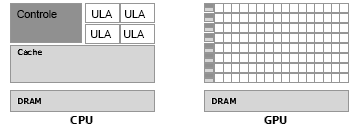
\includegraphics[width=1\textwidth]{imagens/gpu_1.png}
  \caption{As GPUs dedicam mais transistores ao processamento de dados \cite{CUDA}}
  \label{fig:gpu_1}
\end{figure}

Quando surgiram, o foco principal dessas placas era na indústria de jogos. Esse mercado bilionário impulsionou uma rápida evolução na capacidade das GPUs. Não demorou muito tempo para que os desenvolvedores vissem que as potencialidades das GPUs não estavam  limitadas à indústria de jogos. Inicialmente era muito trabalhoso usar a capacidade de processamento das placas de vídeo para aplicações de propósito geral pois era necessário conhecer APIs específicas de processamento de imagem, e saber traduzir os problemas de um domínio para o outro. Para que os desenvolvedores pudessem se aproveitar desse processamento para outros fins, os produtores de GPUs têm disponibilizado bibliotecas para executar operações de uso geral em GPUs, como o CUDA, distribuído pela NVIDIA para ser usado em suas placas gráficas.

\section{CUDA}
Lançado em 2006, CUDA \cite{CUDA} é uma plataforma de computação e um modelo de programação criado pela NVIDIA para que os desenvolvedores possam explorar o potencial das suas GPUs para aplicações de propósito geral. Atualmente, CUDA está na versão 7.5. CUDA foi desenvolvida para ser simples e facilmente compreensível por pessoas com familiaridade com linguagens de programação como C. Com CUDA é possível enviar código em C, C++ e Fortran diretamente para GPU sem precisar escrever em assembly.
%silvana: dizer de outra forma, que neste trabalho usaremos a API de CUDA para a linguagem C.
%Nesse trabalho, não estarei abordando o uso do fortran.
%Felipe: Melhor?
Neste trabalho usaremos a API de CUDA para as linguagens C e C++.
%que foram as linguagens usadas na implementação.

A base do CUDA consiste de 3 abstrações: hierarquia de threads, memória compartilhada e sincronização. Essas abstrações estão acessíveis ao programador através de comandos básicos. 

No modelo de programação de CUDA, as threads (fluxos de execução independente) são organizadas em blocos.
%A execução do CUDA em placa de vídeo é divida em blocos. Blocos são conjuntos de threads (fluxos de execução independente) 
As threads de um mesmo bloco são escalonadas para execução no mesmo núcleo de processamento e compartilham uma área de memória específica de cada núcleo. Dentro de um bloco, as threads são agrupadas em {\em warps} (conjuntos de 32 threads) para serem executadas. Cada warp é um conjunto de threads que executa perfeitamente em paralelo, ou seja, as threads executam ao mesmo tempo a mesma instrução sobre partes distintas do dado de entrada. Em caso de desvio de fluxo dentro de um warp, as threads de fluxos distintos devem aguardar o processamento das demais threads. 

O número de threads por bloco é definido pelo desenvolvedor. É recomendável que o número de threads por bloco seja múltiplo de 32, para aproveitar melhor os warps, mas a configuração que vai dar o melhor resultado, varia de aplicação para aplicação. Atualmente, nenhuma placa de vídeo suporta mais de 1024 threads por bloco, e esse valor precisa ser levado em consideração pelo desenvolvedor. Por exemplo, para executar a soma de dois vetores de 2048 elementos, seria possível configurar 2 blocos de 1024 threads com 32 warps, 4 blocos de 512 threads com 16 warps, ou 64 blocos de 32 threads em um único warp por bloco.

A escalabilidade do CUDA é feita de forma transparente para o desenvolvedor, basta fazer o programa de forma realmente paralela, onde um bloco não precise de informação de outro bloco e a ordem de execução não importe. A execução dos blocos é distribuída em tempo de execução de forma a explorar melhor a arquitetura.

\subsection{Modelo de programação de CUDA}
O núcleo do CUDA consiste de kernels, que são funções especiais compiladas para serem executadas na GPU. O kernel é definido pela declaração \texttt{\_\_global\_\_}. O número de threads e blocos que vai executar a função é especificado quando a função é chamada pela sintaxe \texttt{nomeDaFuncao< < < blocos, threads > > >(parametros...)}.
%Felipe: porque você tinha removido blocos da frase acima?

Para identificar qual thread vai processar qual dado, cada thread possui um identificador de thread, \texttt{threadIdx}, e de bloco, \texttt{blockIdx}, e é possível saber o índice do vetor que se quer acessar fazendo \texttt{indice = threadIdx.x + blockIdx.x * blockDim.x}. O \texttt{.x} serve para identificar a dimensão que estamos acessando, é possivel enviar vetores de até 3 dimensões. A quantidade de threads por bloco na dimensão {\em x} é dada pela variável \texttt{blockDim.x}.
Cada kernel tem acesso à memória privada de cada thread, à memória compartilhada por blocos de threads,  e à memória global compartilhada por todas as threads.

No Código \ref{alg:cuda_1}, apresentamos um exemplo de um kernel que eleva ao quadrado todos os elementos de um vetor. Mostramos como declarar um kernel e como usar o identificador das threads para endereçar a posição correta do vetor que cada thread deve processar.

\codec{Como escrever e invocar um Kernel}{alg:cuda_1}{codigos/cuda_1.txt}

CUDA é um modelo de programação heterogêneo onde parte do programa executa na CPU e outra parte na GPU e cada uma dessas unidades de execução possui sua área de memória.
%. Para isso, cada um executa um código distinto e possui memória distinta. 
Por isso é necessário especificar para a GPU como administrar a memória e quando executar os kernels. O CUDA oferece funções que permitem a CPU dizer para a GPU quando alocar memória, copiar dados para memória da GPU e executar os kernels.

A memória pode ser alocada na GPU através da função \texttt{cudaMalloc(\&dvcPtr, tamanho)}. É preciso salvar a referência do ponteiro da GPU pois é esse ponteiro que vai ser passado para as chamadas de kernel. Para copiar informação do \texttt{host} para o \texttt{device} (GPU), é preciso usar a função \texttt{cudaMemcpy(dvcPtr, hstPtr, tamanho,  tipo)}, onde \texttt{tipo} é um {\em enum} e pode ser \texttt{cudaMemcpyHostToDevice} ou \texttt{cudaMemcpyHostToDevice}, entre outros. Para liberar a memória alocada no \texttt{device}, usa-se \texttt{cudaFree(devicePtr)}. 

As chamadas de CUDA para o \texttt{device} pertencem à um {\em stream} que funciona como uma fila que executa os comandos na ordem que foram chamados. Algumas chamadas, como as de kernel, são por padrão assíncronas em relação ao \texttt{host}. Outras chamadas fazem a CPU eseperar a GPU terminar de trabalhar antes de continuar com o código, como \texttt{cudaMemcpy(...)} e \texttt{cudaDeviceSynchronize()}.

O programa descrito no código \ref{alg:cuda_2} utiliza muito dos conceitos que vimos. Como a alocação de memória no \texttt{device}, a cópia de um vetor do \texttt{host} para o \texttt{device}, a chamada do kernel visto em \ref{alg:cuda_1}, a cópia de um vetor do \texttt{device} para o \texttt{host} e a liberação da memória alocada na GPU.

\codec{Como alocar memória e copiar dados para GPU}{alg:cuda_2}{codigos/cuda_2.txt}

Como as funções de CUDA não executam na CPU, é difícil saber o que está acontecendo, se ocorreu um erro, ou se o programa está em um estado inválido do lado da GPU. Por isso, as funções de CUDA retornam códigos de erro ou sucesso definidos pelo {\em enum }\texttt{cudaError}. O kernel não possui esse retorno, então é necessário checar o estado da GPU após as chamadas de kernel para saber se ocorreu algum erro.  A função \texttt{cudaGetLastError()} pode ser usada para fazer essa verificação.

É possível incluir funções dentro de kernels de CUDA. Para isso é preciso colocar a diretiva \texttt{\_\_device\_\_} na assinatura da função. Dessa forma, o compilador saberá que essa função deve ser executada na GPU e para isso irá gerar o código de máquina adequado. Caso queira que a função também possa executar na CPU, é possível colocar a diretiva \texttt{\_\_host\_\_}. Assim, usando as duas diretivas é possível invocar a mesma função em códigos dentro e fora de kernels de CUDA.

\chapter{Desenvolvimento}\label{chp:LABEL_CHP_4}

A linguagem escolhida para o desenvolvimento foi o c++ pois possui boa performance e possui muitos exemplos de CUDA disponível no CUDA ToolKit 7.5 \cite{CUDA}. As ferramentas Visual Studio 2013, IDE desenvolvida pela Microsoft, e Rasharper c++, plugin desenvolvido pela JetBrains, foram usadas para facilitar o desenvolvimento. Juntas essas ferramentas oferecem muitas funcionalidades de navegar pelo código, refatoramento, debug e Testes Automatizados. Para o controle de versão foi usado o Git e todo o código fonte incluindo o latex desse relatório se encontram em \url{https://github.com/felipesfaria/FariaTcc}.

\section{Comandos do Programa}
O programa foi feito de forma que alguns parâmetros possam ser recebidos pela linha de comando. 
Esses parâmetros são carregados no inicio do programa pela classe \texttt{Settings}.
Se rodar o programa sem comandos todos os parâmetros tem definido um valor default e também é possível enviar o comando -h para ver na tela os comandos possíveis.

\begin{table}
    \small
    \centering
    \begin{tabular}{c|c|c|c}
        Comando & Descrição & Tipo / Valores aceitos & Default \\ \hline
        -c & Constante de margem flexível & double & 999.0 \\ \hline
        -d & Conjunto de Dados &  i:Iris & i \\ 
         &  &  a[1-9]:Adult &  \\ 
         &  &  w[1-8]:Web &  \\ \hline
        -f & Partições na validação cruzada & int & 10 \\ \hline
        -g & $\gamma$ usado pelo kernel gaussiano & double & 0.5 \\ \hline
        -h & Menu de ajuda & & \\ \hline
        -l & Nível de log & a:Todos , r:Resultados  & r \\
           & & e:Erros , n:Nenhum & \\ \hline
        -mi & Máximo de Iterações & int & 128 \\ \hline
        -p & Precisão da parada & double & 1e-010 \\ \hline
        -sd & Gerador de numero aleatório & int & time(nullptr) \\ \hline
        -st & Paço inicial & double & 1 \\ \hline
        -svm & Tipo de MVS & p:Paralelo & s \\
         &  & s:Sequencial &  \\ \hline
        -t & Threads por Bloco & int & 128 \\
    \end{tabular}
    \caption{Comandos aceitos pelo programa}
    \label{tab:commands}
\end{table}

\section{Estrutura de Dados}
Desenvolvemos o programa para ler arquivos no mesmo formato que os conjuntos de dados apresentados no site do LIBSVM \cite{art:LIBSVM}. Esse formato consiste em apresentar primeiro a classe da amostra representada por um numero, seguida por seus atributos no formato \texttt{indice:valor}, como podemos ver no exemplo \ref{alg:datasample} temos um conjunto de dados com 4 amostras, duas de cada classe, cada uma com 4 atributos.

\codec{Conjunto de dados no formato do LIBSVM}{alg:datasample}{codigos/datasample.txt}

A leitura do arquivo com o conjunto de dados é feita pela classe \texttt{DataSet}. Os atributos das amostras são salvos em \texttt{vector<vector<double>> X} e as suas classes em \texttt{vector<double> Y}.

Para se obter as métricas usadas na avaliação é usado um método conhecido como validação cruzada onde o conjunto de dados é dividido em $n$ partições. Para cada partição $i \in [1,n]$ é feita um treinamento com as outras partições $[1,n]-i$ em seguida é feita a classificação de todas as amostras na partição $i$ para conseguir um resultado de performance para esse conjunto de treinamento e validação. Isso é feito para todos os conjuntos de $n$ de forma que todas as amostras foram classificadas uma vez e participaram de $n-1$ treinamentos, dessa forma conseguimos $n$ avaliações disjuntas de precisão da MVS e uma boa analise de desempenho minimizando os impactos externos que poderiam afetar apenas uma execução.

Para dividir o conjunto de dados em treinamento e avaliação utilizo as classes \texttt{TrainingSet} e \texttt{ValidationSet} que herdam de \texttt{BaseSet}. \texttt{BaseSet} possui um conjunto de dados armazenando as amostras em \texttt{double* x}, as classes em \texttt{double* y}, \texttt{int width} é a quantidade de argumentos e \texttt{int height} é o numero de amostras no conjunto. \texttt{void BaseSet::Init(int height, int width)} define \texttt{height} e \texttt{width} e aloca memória para \texttt{x} e \texttt{y}. As amostras em \texttt{x} são salvas em um único vetor continuo e podem ser endereçadas por \texttt{indiceReal = indiceDaAmostra*width}.
Além dos atributos em \texttt{BaseSet}, \texttt{TrainingSet} possui os valores de $\alpha$ em \texttt{double* alpha} descobertos no treinamento para serem usados na classificação, e \texttt{ValidationSet} mantem a quantidade de classificações corretas para análise posterior.
Esses objetos são inicializados a partir do método \texttt{void InitFoldSets(TrainingSet *ts, ValidationSet *vs, int fold)}, onde cada conjunto é definido pela função \texttt{void InitFoldSets(TrainingSet *ts, ValidationSet *vs, int fold)} apresentada em \ref{alg:InitFoldSet}.

\codec{Como dividir o conjunto de dados para validação cruzada}{alg:InitFoldSet}{codigos/InitFoldSet.txt}

\section{Kernel Gaussiano}
Para implementar o algoritmo \ref{alg:KAA} é preciso levar algumas coisas em consideração. O primeiro seria como fazer o Kernel? Inicialmente desenvolvemos a aplicação de forma que implementasse todos os algoritmos listados na tabela \ref{tab:Kernels}, mas logo nas primeiras versões vimos que os resultados com o kernel Gaussiano estavam melhores que os outros, além disso todas as referências, citadas em \ref{chp:LABEL_CHP_1} usaram apenas o kernel gaussiano. Por isso implementamos somente o kernel gaussiano de forma a reduzir o escopo de análise.

O kernel gaussiano é definido como $k(\bar{x},\bar{y})=e^{-\big(\frac{|\bar{x}-\bar{y}|^2}{2\sigma^2}\big)}$, para economizar cálculos fazemos algumas simplificações. Substituímos $\frac{1}{2\sigma^2}$ por $\gamma$ que é calculado quando o valor é definido na inicialização do programa. Como $|\bar{x}| = \sqrt{\sum x_i^2}$ podemos simplificar $|\bar{x}-\bar{y}|^2 = \bigg(\sqrt{\sum (x_i-y_i)^2}\bigg)^2=\sum (x_i-y_i)^2$. A função que programamos no final é equivalente à $e^{\big(-\gamma*\sum (x_i-y_i)^2\big)}$.
Para garantir que a versão sequencial e paralela funcionam da mesma forma e para evitar a repetição de código definimos a função de kernel gaussiano com as diretivas \texttt{\_\_host\_\_} e \texttt{\_\_device\_\_}, como pode ser visto no código \ref{alg:gaussKernel}.

\codec{Kernel Gaussiano}{alg:gaussKernel}{codigos/gaussKernel.txt}

\section{Maquinas de Vetores de Suporte}
Mais uma vez para evitar repetição de código e para utilizar melhor as propriedades do C++ definimos a classe \texttt{BaseSvm} com os métodos \texttt{virtual void Train(TrainingSet *ts)} e \texttt{virtual void Test(TrainingSet *ts, ValidationSet *vs)}, assim é possível definir no código toda a execução do programa só precisando especificar no gerador do MVS qual tipo vamos usar, depois disso desenvolvemos duas classes que herdam de \texttt{BaseSvm}, \texttt{ParallelSvm} e \texttt{SequentialSvm}.

Programar o algoritmo Kernel-Adatron \ref{alg:KAA} é simples. Porem alguns pontos precisam ser revistos. A condição de parada e o valor de $\eta$. Existem conjuntos de dados difíceis de se calcular que pode fazer com que o programa rode por uma quantidade de tempo considerável. Para isso definimos um limite máximo de iterações que pode ser definido por \texttt{-mi}, seu valor default é \texttt{512}. Outra abstração abordada na implementação está em $\bar{\alpha}-\bar{\alpha_{old}}\approx \bar{0}$. Precisamos definir o quão próximo de zero é o suficiente para nosso programa. Com essa precisão $p$ nós definimos que $a\approx b$ se $|a-b|<p$. Esse parâmetro pode ser configurado por \texttt{-p} e o valor padrão é \texttt{1e-5}. Assim nossa condição de parada fica \texttt{abs(avgDif) > Precision \&\& count < MaxIterations}, onde \texttt{avgDif} é a media de $\bar{\alpha}-\bar{\alpha_{old}}$ e \texttt{count} é o numero de iterações.

Embora na seção \ref{sec:kaa} tenhamos visto que o algoritmo sempre irá convergir dado um $\eta$ pequeno o suficiente, esse tamanho é difícil de se descobrir. Se for muito grande o algoritmo pode nunca convergir e sempre ultrapassar o ponto ótimo. Se for muito pequeno o algoritmo pode demorar muito para chegar no ponto ótimo. A solução encontrada para o problema foi adotar um $\eta$ flexível. Começando com um valor grande, sempre que percebemos que passamos do ponto ótimo reduzimos $\eta$ na metade. Assim não corremos o risco de arbitrariamente escolher um valor ruim. Permitimos que o valor inicial de $\eta$ seja definido por linha de comando com o comando \texttt{-s} e o default é \texttt{1} como pode ser visto na tabela \ref{tab:commands}.

Agora precisamos considerar como sabemos que passamos do ponto para reduzir o valor de $\eta$. Para isso fazemos dois testes. Primeiro vemos se nos afastamos do ponto ótimo, checando se o valor de \texttt{avgDif} aumentou. Depois vemos se o sinal de \texttt{avgDif} mudou, se ele era crescente e virou decrescente ou se ele era decrescente e virou crescente significa que o gradiente mudou de direção. Isso é feito no função mostrada em  \ref{alg:updateStep}

\codec{Atualização de $\eta$}{alg:updateStep}{codigos/updateStep.txt}

Percebemos na pratica que alguns parametros convergem mais rapidos que outros. Por isso implementamos dois métodos diferentes de atualização de $\eta$. Um em que só possuimos um valor de $\eta$ aplicado em todos os valores de $\alpha_i$ e outro em que utilizamos um vetor $\bar{\eta}$ onde possuimos um valor de $\eta_i$ para cada $\alpha_i$. Chamamos isso de \texttt{StepMode} que pode ser \texttt{SingleStep} ("s") ou \texttt{MultiStep} ("m") na linha de comando com \texttt{-sm}.

No algoritmo Kernel-Adatron visto os valores de alpha são usados assim que são descobertos. Essa versão é conhecida como Kernel-Adatron estocástico. Já que na nossa versão paralela nãos erá possivel implementar o método estocástico já que calcularemos todos os valores de $\alpha$ paralelamente implementamos as duas versões na forma sequencial. É possivel definir pelo comando \texttt{-ua} se o valor de $\alpha_i$ vai ser atualizado assim que descoberto definimos \texttt{-ua t}, o padrão que utilizamos ou \texttt{-ua f} faz com que os valores de alpha sejam atualizados simultaneamente ao final de cada iteração. No capitulo \ref{chp:LABEL_CHP_5} avaliamos qual forma funciona melhor.

Podemos ver como ficou o loop principal da função de treinamento sequencial em \ref{alg:SequentialSvmTrain}.

\codec{Treinamento Sequencial}{alg:SequentialSvmTrain}{codigos/SequentialSvmTrain.txt}

A função de classificação pode ser implementada diretamente da equação matemática sem muita complicação. Utilizamos o $\bar{\alpha}$ encontrado no treinamento e $\bar{x}$ que está armazenado no \texttt{TrainingSet} para descobrir a classe do exemplo de validação.

\codec{Classificação Sequencial}{alg:SequentialSvmClassify}{codigos/SequentialSvmClassify.txt}

\section{Paralelização}


\chapter{Avaliação} \label{chp:LABEL_CHP_5}

A avaliação de um classificador paralelo é complicada. É necessário levar em consideração tanto a performance em precisão quanto em velocidade, e melhorar um sem piorar o outro. Maquinas de suporte de vetores possuem diversos parâmetros que alteram tanto a precisão quanto a velocidade do programa em versão paralela e sequencial. Todos os conjuntos de dados estão disponíveis tanto no site do UCI \cite{UCI} quanto no site do LIBSVM \cite{art:LIBSVM}.

\section{Conjunto de Dados}\label{sec:LABEL_CHP_5_SEC_A}
Antes de analisar os resultados, devemos analisar os conjuntos de dados estudados.
\subsection{Iris} \label{sec:Iris}
Originalmente esse conjunto de dados distinguia entre 3 tipos de iris, uma especie de flor, os atributos descrevem os tamanhos das pétalas e das sépalas. São 150 amostras no conjunto.
\subsection{Adult} \label{sec:Adult}
O objetivo desse conjunto de dados é analisar a faixa de renda de um adulto americano baseado em diversos fatores. A classificação prevê se o individuo tem renda de mais ou menos que 50 mil dólares por ano. Alguns dos atributos são idade, pais de origem, etnia, estado civil e escolaridade. Existem 9 versões desse conjunto de dados variando o numero de amostras entre 1,605 e 32,561.
\subsection{Web} \label{sec:Web}
Esse conjunto de dados determina se uma pagina pertence a uma categoria ou não baseado na presença de palavras chave. Existem 8 versões desse conjunto de dados variando o numero de amostras entre 2,477 e 49,749.

\subsection{Tratamento dos dados}
No conjunto \ref{sec:Iris}, foi necessário remover uma das classes para que o conjunto fosse compatível o classificador binário. As duas classes remanescentes são linearmente separáveis de forma que o conjunto serviu para facilitar os testes no inicio do desenvolvimento.

Os conjuntos \ref{sec:Adult} e \ref{sec:Web} possuem atributos multi-variados, atributos que são definidos por uma classe, como por exemplo $PaisDeOrigem \in \left [ Brasil,Espanha,Noruega \right ]$. É preciso atribuir valores numéricos para esses atributos para que funcionem com a maquina de vetores de suporte. Para isso trocamos os atributos multi-variados por valores binários. Substitui-se o atributo $PaisDeOrigem$, por 3 atributos binários que podem ser verdadeiro ou falso, $Brasileiro \in \left [ 0,1 \right ]$, $Espanhol \in \left [ 0,1 \right ]$ e $Noruegues \in \left [ 0,1 \right ]$. Essas parametrizações já estavam feitas no site do LIBVSM.

%\section{Performance Tempo}\label{sec:LABEL_CHP_5_SEC_B}

%\section{Performance Precisão}\label{sec:LABEL_CHP_5_SEC_C}
\chapter{Conclusão}\label{chp:LABEL_CHP_6}

%silvana: acho melhor começar com uma síntese do objetivo do trabalho...
%silvana: frase muito grande...
%Felipe: Melhor?
%Nosso objetivo inicial 
Nesse trabalho, desenvolvemos uma versão sequencial e uma versão paralela de uma máquina de vetores suporte usando o algoritmo Kernel-Adatron. Para a paralelização escolhemos a GPU e fizemos isso usando a plataforma CUDA.
%Ao entendermos a teoria por trás da 
Máquina de vetores suporte é uma técnica de aprendizado de máquina que projeta dados de problemas que não são linearmente separáveis em um espaço de dimensão maior onde eles podem ser separados. Para separá-los usamos o hiperplano separador que é encontrado resolvendo a dual lagrangiana desse problema, de forma que nosso resultado é um vetor $\bar{\alpha}$. O algoritmo Kernel-Adatron atualiza todos os elementos desse vetor com o seu gradiente em diversas iterações até chegar no seu valor ótimo.

As GPUs que evoluíram para processar imagens e renderizar objetos em 3 dimensões tem uma alta capacidade de paralelização, com vários núcleos capazes de executar instruções em vários elementos distintos de um vetor. A CUDA é uma plataforma de programação da NVIDIA que permite que desenvolvedores explorem esse potencial em aplicações que não são relacionados à computação gráfica.

Neste trabalho exploramos a capacidade de processamento paralelo das GPUs para reduzir o tempo de execução do algoritmo Kernel-Adatron. A versão desse algoritmo que vimos em \cite{art:LIVRO_KAA} adotava um modelo estocástico, que não era viável na versão paralela pois possui uma dependência no laço principal do algoritmo. Por isso implementamos uma versão sequencial estocástica e não estocástica e vimos que elas alcançam a mesma porcentagem de acertos.

Ao comparar nossa versão com o LIBSVM, vimos que alcançamos porcentagens de acertos bastante próximas. Em tempo de execução ainda estamos longe, o que mostra o quão avançado o SMO é em relação ao Kernel-Adatron.

Para medir a qualidade da nossa paralelização, comparamos nossa versão sequencial com a paralela. A porcentagem de acertos ficou próxima, variando em menos de 1\% em alguns casos e sendo exatamente igual na maioria. Ao comparar o tempo de execução do programa entre as versões conseguimos um speedup de duas até seis vezes melhor.

\section{Trabalhos Futuros}

Separamos as melhorias que poderiam ser feitas em nosso programa em duas seções. As melhorias na máquina de vetores suporte, que consistem em aplicar técnicas mais avançadas de MVS; % para obtermos nossos resultados 
e as melhorias na implementação paralela que seriam formas de utilizar melhor os recursos da GPU.

Além dessas melhorias poderiam ser feitos mais experimentos. Analisando, por exemplo, os conjuntos maiores para descobrir quais parâmetros dariam um melhor resultado para esses conjuntos.
%Silvana: explicar quais experimentos e com qual finalidade.


\subsection{Melhorias na MVS}

Fazer a máquina de vetores suporte multi-classe é relativamente simples a partir de uma máquina de vetores suporte binária, como o Kernel-Adatron. Para isso é necessário quebrar a classificação em problema menores. Em vez de treinar apenas uma MVS se treina uma MVS para cada classe, que vai aprender se um exemplo é ou não dessa classe. Como no final são feitas várias classificações diferentes isso poderia ser feito externamente à paralelização.

Além disso, é possível modificar o algoritmo Kernel-Adatron para fazer regressão ao invés de classificação. Este processo é fácil de se encontrar e está descrito em \cite{art:LIVRO_KAA}.

\subsection{Melhorias na implementação paralela em GPU} \label{sec:melhoriasCuda}

Como foi mencionado por \cite{art:REF_ART_2}, GPUs possuem mais unidades lógicas de float do que de double. Seria interessante modificar o programa para usar os dois tipos para comparar sua execução.

Na nossa implementação só usamos a memória global, um aproveitamento maior da hierarquia de memória da GPU no nosso programa poderia aumentar muito o speedup encontrado. Um primeiro experimento desse tipo poderia ser feito usando a memória compartilhada, que é visível para todas as threads dentro de um bloco e requer tempo de acesso menor que a memória global. Podemos nos aproveitar do fato que cada thread atualiza um $\alpha_i$ e usa o mesmo $\bar{x}_i$ em todas suas iterações. Considerando que $C$ é o conjunto de índices de $\alpha_i$ que são atualizados por um bloco, se copiarmos todos os exemplos $\bar{x}_i\quad|\quad i\in C$ para a memória compartilhada já poderíamos ter um ganho no speedup.

Em diversas partes do algoritmo precisamos do somatório dos valores de um vetor, como para medir a condição de parada no treinamento e para descobrir o sinal da função de classificação. Na nossa implementação isso é feito de forma sequencial na CPU. Entretanto, existem algoritmos bem definidos e eficientes de somatório de vetores em GPU que poderiam ser implementados, como o algoritmo descrito por Mark Harris em \cite{harris2007optimizing}.

\pagebreak

%%%%%%%%%%%%%%%%%%%%%%%%%%%%%%%%%%%%%%%%%%%%%%%%%%%%%%%%%%%%
% B I B L I O G R A F I A
%%%%%%%%%%%%%%%%%%%%%%%%%%%%%%%%%%%%%%%%%%%%%%%%%%%%%%%%%%%%
% Retirar esta parte se o trabalho não tiver bibliografia
\makebibspage{apalike}{elementos-postextuais/referencias}

%%%%%%%%%%%%%%%%%%%%%%%%%%%%%%%%%%%%%%%%%%%%%%%%%%%%%%%%%%%%
% A P E N D I C E
%%%%%%%%%%%%%%%%%%%%%%%%%%%%%%%%%%%%%%%%%%%%%%%%%%%%%%%%%%%%
% Retirar esta parte se o trabalho não tiver anexos
%\appendix
%\chapter{Lorem ipsum dolor sit amet}\label{chp:LABEL_APP_1}

Lorem ipsum dolor sit amet, consectetur adipiscing elit. Donec lacus nisl, ultricies vitae semper eu, scelerisque nec enim. Curabitur posuere tortor orci, at porta leo laoreet et. Quisque ut congue dolor. Maecenas vel sagittis diam. Praesent fermentum eleifend mi, sit amet vehicula leo pellentesque quis. Curabitur mattis luctus pulvinar. Proin auctor est nec nulla pellentesque commodo. Donec nec justo eu magna aliquet eleifend. Curabitur tristique tortor id sem dignissim, a iaculis metus interdum. Phasellus bibendum velit sit amet interdum semper. Nam vestibulum dui quis nisi consectetur, id vehicula dolor faucibus.

\end{document}